\documentclass[aspectratio=169,11pt]{beamer}
% ==========================================================================
%  KSA lecture-slide theme  =  stock beamer "Boadilla"  +  KSA colour theme
%  brand colours sampled from the official KSA symbol mark:
%    Deep Prussian Blue  #2E3192   (지성 - intellect)
%    Golden Gray         #D6CBB1   (감성 - sensibility)
%  Engine: XeLaTeX.  Usage:
%    \documentclass[aspectratio=169,11pt]{beamer}
%    \input{../../theme/ksa-theme.tex}
%  Each deck lives in its own slides/kor/<deck>/ folder together with its
%  own images; ../../figs/ is kept only as a fallback for the shared cache.
% ==========================================================================

\usepackage{fontspec}
\usepackage{amsmath,amssymb}
\usepackage{graphicx}
\graphicspath{{figs/}{./}{../../../figs/}}
\usepackage{booktabs}
\usepackage{listings}
\usepackage{varwidth}

% ---- fonts (no ctex/xeCJK on this box -> fontspec drives CJK directly) -----
\defaultfontfeatures{Ligatures=TeX}
\setmainfont{Noto Sans CJK KR}
\setsansfont{Noto Sans CJK KR}
\setmonofont{Noto Sans Mono CJK KR}[Scale=0.92]

% ---- base theme: stock Boadilla ------------------------------------------
\usetheme{Boadilla}
\usefonttheme{professionalfonts}
\setbeamertemplate{navigation symbols}{}

% ---- KSA colour theme (recolour the stock theme) --------------------------
\definecolor{ksablue}{HTML}{2E3192}
\definecolor{ksabluedk}{HTML}{20226A}
\definecolor{ksagold}{HTML}{D6CBB1}
\definecolor{ksagolddk}{HTML}{A9976B}
\definecolor{ksared}{HTML}{C0392B}
\definecolor{ksagray}{HTML}{5B5B5B}

\setbeamercolor{structure}{fg=ksablue}
\setbeamercolor{alerted text}{fg=ksared}

\setbeamercolor{palette primary}{fg=white,           bg=ksablue}
\setbeamercolor{palette secondary}{fg=white,         bg=ksablue!85!black}
\setbeamercolor{palette tertiary}{fg=white,          bg=ksabluedk}
\setbeamercolor{titlelike}{fg=ksablue}
\setbeamercolor{frametitle}{fg=ksablue,bg=}
\setbeamercolor{title}{fg=ksablue}
\setbeamercolor{author}{fg=ksagray}
\setbeamercolor{institute}{fg=ksagray}
\setbeamercolor{block title}{fg=white,bg=ksablue}
\setbeamercolor{block body}{fg=black!85,bg=ksablue!6}
\setbeamercolor{item}{fg=ksablue}
\setbeamercolor{section in toc}{fg=black!85}

\setbeamerfont{frametitle}{series=\bfseries}
\setbeamerfont{title}{series=\bfseries}

% ---- footline:  KSA mark | "Made by ..." | n / N   (matches reference) ----
\newcommand{\ksacredit}{}
\setbeamertemplate{footline}{%
  \hbox{%
    \begin{beamercolorbox}[wd=.18\paperwidth,ht=2.6ex,dp=1.5ex,leftskip=1.1em]{}%
      \raisebox{-0.35ex}{\includegraphics[height=2.0ex]{ksa-logo.png}}%
    \end{beamercolorbox}%
    \begin{beamercolorbox}[wd=.64\paperwidth,ht=2.6ex,dp=1.5ex,center]{}%
      {\scriptsize\color{ksagray}\ksacredit}%
    \end{beamercolorbox}%
    \begin{beamercolorbox}[wd=.18\paperwidth,ht=2.6ex,dp=1.5ex,rightskip=1.1em]{}%
      \hfill{\scriptsize\color{ksablue}\insertframenumber\,/\,\inserttotalframenumber}%
    \end{beamercolorbox}%
  }%
  \vskip2pt
}

% ---- section divider: stock \sectionpage, KSA-coloured -------------------
\setbeamertemplate{section page}{%
  \begingroup\centering
    {\color{ksagolddk}\rule{0.16\paperwidth}{1pt}}\par\vskip1.0em
    {\usebeamerfont{title}\color{ksablue}\insertsectionhead\par}\vskip1.0em
    {\color{ksagolddk}\rule{0.16\paperwidth}{1pt}}\par
  \endgroup
}
\AtBeginSection[]{\begin{frame}[plain,noframenumbering]\vfill\sectionpage\vfill\end{frame}}

% ---- code listings ------------------------------------------------------------
\lstdefinestyle{ksa}{%
  basicstyle=\ttfamily\scriptsize,
  keywordstyle=\color{ksablue}\bfseries,
  commentstyle=\color{ksagray}\itshape,
  stringstyle=\color{ksagolddk},
  numberstyle=\tiny\color{ksagray},
  backgroundcolor=\color{ksablue!6},
  frame=leftline, framerule=1.4pt, rulecolor=\color{ksablue},
  xleftmargin=1em, aboveskip=0.8em, belowskip=0.4em,
  showstringspaces=false, breaklines=true, language=Python,
}
\lstset{style=ksa}

% ---- handy macros -----------------------------------------------------------
\newcommand{\kb}[1]{\textbf{\color{ksablue}#1}}   % blue keyword
\newcommand{\kq}[1]{\textbf{\color{ksared}#1}}    % red key-question

\setbeamerfont{title}{series=\bfseries,size=\fontsize{24}{30}\selectfont}
\setbeamerfont{subtitle}{series=\bfseries,size=\fontsize{14}{18}\selectfont}
\setbeamerfont{author}{size=\normalsize}
\setbeamerfont{institute}{size=\small}
\graphicspath{{figs/}{../../../../assets/}}
\makeatletter
\newcommand{\markpage}[1]{\protected@write\@auxout{}{\string\newlabel{#1}{{\the\c@framenumber}{}}}\hypertarget{#1}{}}
\newcommand{\pref}[1]{\hyperlink{#1}{\textcolor{ksagolddk}{(p.\ref{#1})}}}
\makeatother

\renewcommand{\ksacredit}{Machine Learning 1 \,\textperiodcentered\, 임베딩}
\title{표상과 임베딩 (Representation · Embedding)}
\subtitle{세상을 숫자 공간의 한 점으로}
\author{Machine Learning 1}
\institute{한국과학영재학교 (KSA)}
\date{}
\begin{document}
\begin{frame}[plain,noframenumbering]\titlepage\end{frame}


% --- 오늘의 질문
\begin{frame}{``세계는 나의 표상이다''}
\vfill
\begin{columns}[c]
\column{0.3\linewidth}\centering
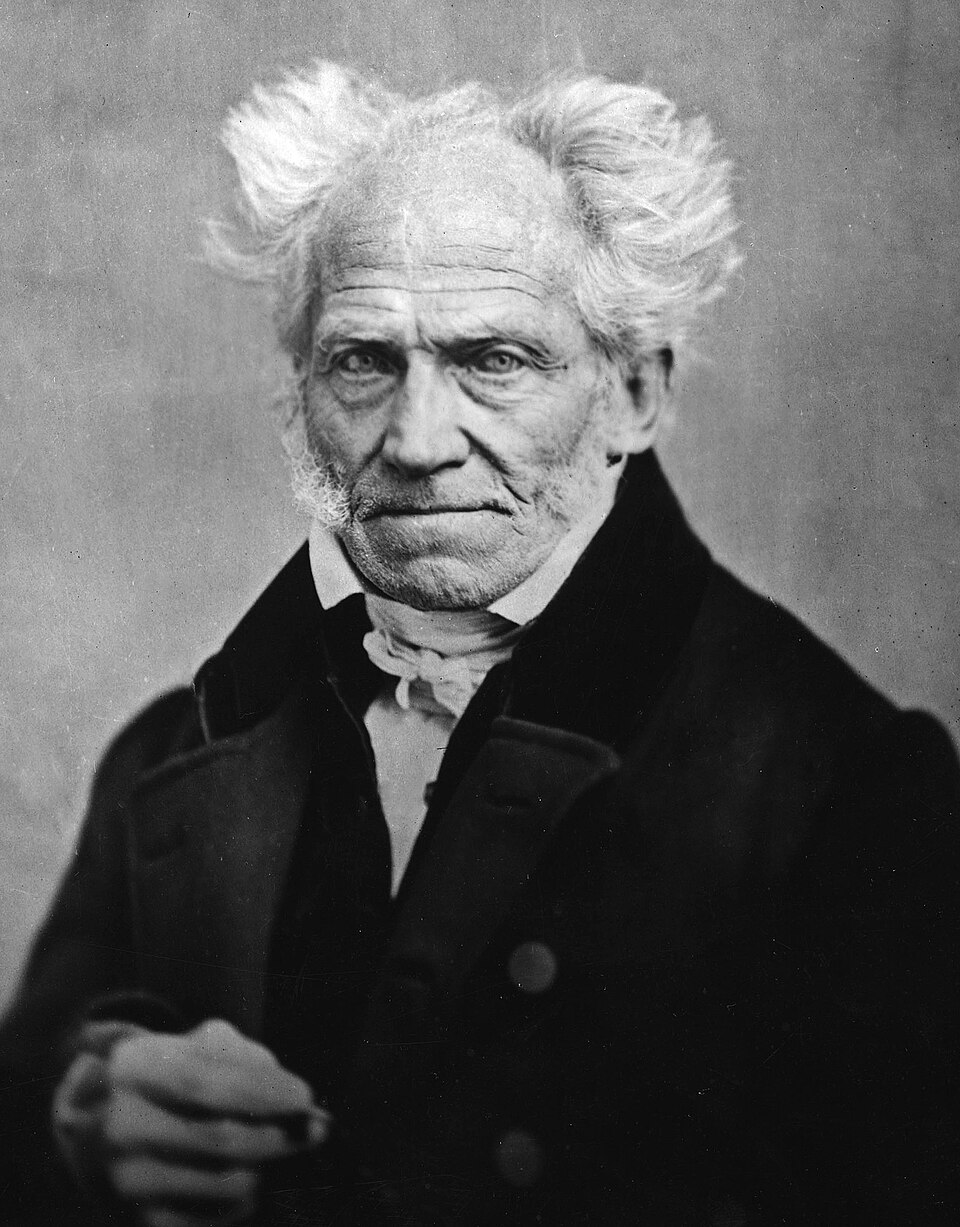
\includegraphics[width=0.85\linewidth]{schopenhauer_1859.jpg}\\
{\small 쇼펜하우어 (1859)}
\column{0.66\linewidth}
{\large 『의지와 표상으로서의 세계』 (1819) 첫 문장}\\[0.8em]
{\large 표상 = re (다시) + presentation (보여 주기)}\\[0.4em]
{\large 생각은 세상을 머릿속에 \textbf{다시 보여 주는} 것}\\[0.8em]
{\large 신경망은 세상을 무엇으로 다시 보여 줄까? \quad $\to$ \kb{숫자 벡터}}
\end{columns}
\vfill
\note{세계는 나의 표상이다. 철학자 쇼펜하우어가 1819년에 낸 책의 첫 문장입니다. 표상, representation은 다시라는 re와 보여 주기라는 presentation이 합쳐진 말입니다. 심리학에서는 생각을, 세상을 머릿속에 다시 보여 주는 표상이라고 합니다. 그렇다면 신경망은 세상을 무엇으로 다시 보여 줄까요? 숫자 벡터입니다. 오늘은 이 숫자 벡터, 임베딩을 정리합니다.}
\end{frame}

% --- 정의
\begin{frame}{임베딩: 대상을 숫자 공간의 한 점으로}
\vfill
\centering
{\large embed = (어딘가에) 끼워 넣다, 박아 넣다 \quad $\to$ \textbf{embedded representation}}\vskip0.8em
\renewcommand{\arraystretch}{1.5}
{\large\begin{tabular}{lll}
지금까지 본 임베딩 & 대상 & 어떻게 만들었나\\\hline
word2vec (14주차) & 단어 & 주변 단어 맞히기\\
GCN (13주차) & 노드 (사람) & 이웃 평균 + 분류\\
CNN 중간층 (10주차) & 사진 & 분류 학습의 부산물\\
트랜스포머 입력 (12주차) & 토큰 & 단어 표 + 위치
\end{tabular}}\vskip0.6em
{\large 좋은 임베딩: \kb{닮은 것은 가깝게}, 다른 것은 멀게}
\vfill
\note{embed는 끼워 넣다, 박아 넣다라는 뜻입니다. 대상을 숫자 공간의 한 점으로 박아 넣은 표상, embedded representation을 줄여 임베딩이라고 합니다. 사실 지금까지 여러 번 봤습니다. word2vec은 단어를, GCN은 사람 같은 노드를, CNN의 중간층은 사진을, 트랜스포머의 입력층은 토큰을 벡터로 바꿨습니다. 좋은 임베딩은 닮은 것은 가깝게, 다른 것은 멀게 둡니다.}
\end{frame}

% --- 표 찾기
\begin{frame}{가장 단순한 임베딩: 표에서 한 줄 꺼내기}
\markpage{lookup}
\vfill
\centering
{\Large\[ \underbrace{(0,\ 0,\ 1,\ 0)}_{\text{3번째 단어 (원-핫)}} \begin{pmatrix} 0.2 & 0.9 \\ 0.8 & 0.1 \\ \mathbf{0.7} & \mathbf{0.3} \\ 0.1 & 0.6 \end{pmatrix} = \kb{(0.7,\ 0.3)} \]}\vskip0.4em
{\large 원-핫 × 표 $W$ = 표의 \textbf{3번째 줄} \quad $\to$ 곱셈 대신 줄을 꺼내면 된다 (\texttt{nn.Embedding})}\\[0.4em]
{\large 표 $W$ 의 숫자는 처음엔 무작위, 학습하면서 \textbf{과제에 맞게} 바뀐다}\\[0.2em]
{\small BERT: 단어 약 3만 개 × 768칸 = 약 2,300만 개 숫자가 이 표 하나}
\vfill
\note{가장 단순한 임베딩은 표에서 한 줄을 꺼내는 겁니다. 단어가 4개, 벡터가 2칸이면 4 곱하기 2 표 W가 있고, 3번째 단어의 원-핫 벡터 0, 0, 1, 0에 W를 곱하면 표의 3번째 줄, 0.7, 0.3이 나옵니다. 그래서 실제로는 곱셈 대신 줄을 꺼냅니다. PyTorch의 nn.Embedding이 이겁니다. 표의 숫자는 처음엔 무작위이고, 학습하면서 과제에 맞게 바뀝니다. BERT는 단어 약 3만 개에 768칸이라, 이 표 하나에 약 2300만 개의 숫자가 있습니다.}
\end{frame}

% --- 실험 1
\begin{frame}{실험 1: 고양이 vs 개만 배운 신경망}
\markpage{exp1}
\vfill
\centering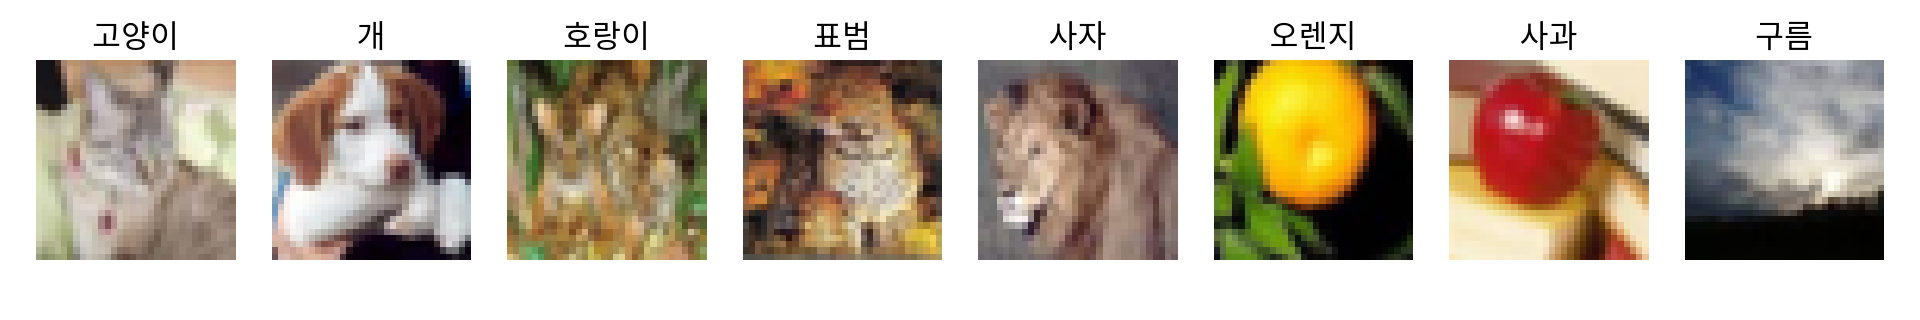
\includegraphics[width=0.86\linewidth]{emb_samples.png}\par\vskip0.2em
\begin{columns}[c]
\column{0.5\linewidth}\centering
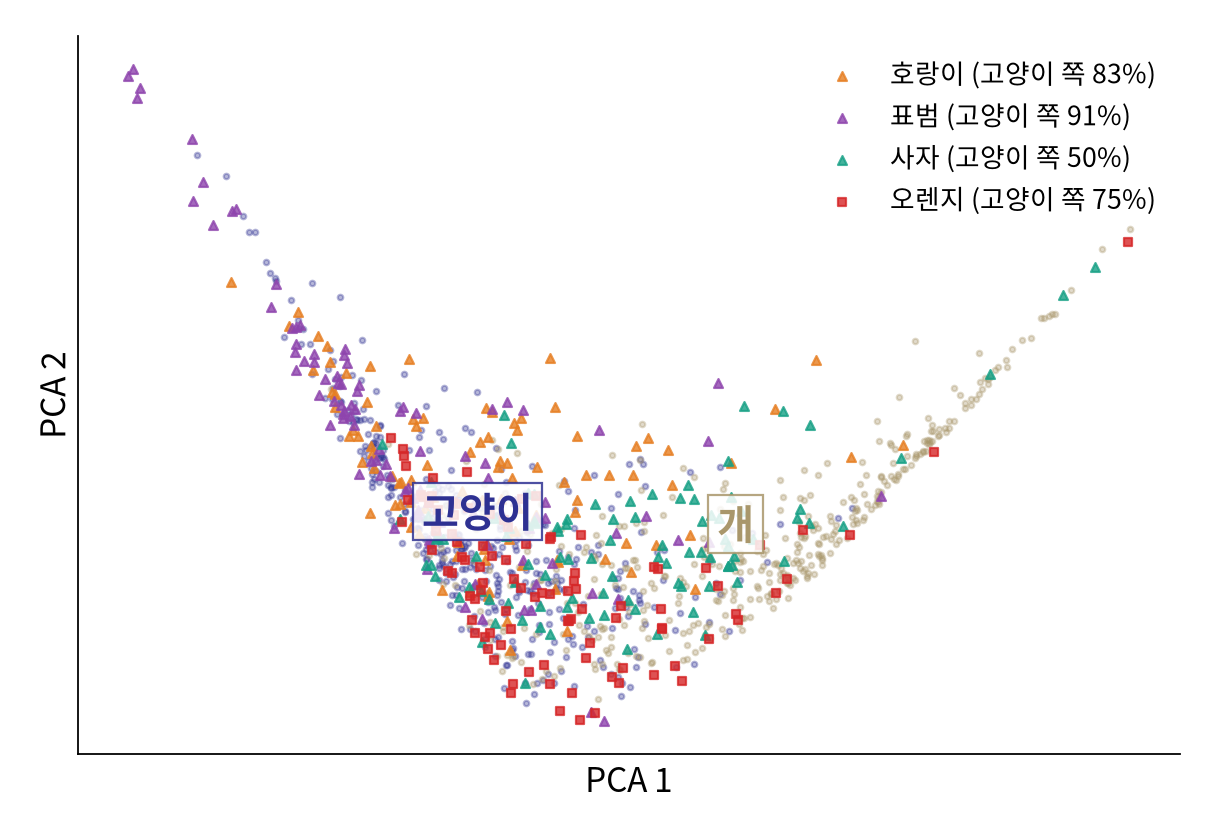
\includegraphics[width=\linewidth]{emb_cnn_map.png}
\column{0.48\linewidth}
{\large CIFAR-10 고양이 · 개 1만 장, 작은 CNN}\\{\large 시험 정확도 \kb{84.1\%}}\\[0.5em]
{\large 마지막 은닉층 64칸 = 임베딩}\\[0.5em]
{\large 처음 보는 사진 (CIFAR-100):}\\
{\large 호랑이 \kb{83\%} · 표범 \kb{91\%} 가 고양이 쪽}\\
{\large 사자는 \kq{50\%}: 반반}
\end{columns}
\vfill
\note{첫 번째 실험입니다. CIFAR-10의 고양이와 개 사진 1만 장으로 작은 CNN을 학습했습니다. 시험 정확도는 84.1퍼센트입니다. 마지막 은닉층의 64칸 벡터를 임베딩으로 보고, 한 번도 보여 준 적 없는 CIFAR-100의 호랑이, 표범, 사자, 오렌지 사진을 넣어 봤습니다. 고양이 중심과 개 중심 중 어디에 더 가까운지 재면, 호랑이는 83퍼센트, 표범은 91퍼센트가 고양이 쪽입니다. 고양잇과의 생김새를 잡아낸 거죠. 사자는 반반입니다. 갈기 때문인지 개와도 닮아 보이나 봅니다.}
\end{frame}

% --- 오렌지
\begin{frame}{그런데 오렌지는? 배운 만큼만 보인다}
\vfill
\centering
\renewcommand{\arraystretch}{1.4}
{\large\begin{tabular}{lccc}
 & 고양이 쪽 & 고양이 · 개가 안 쓰는 칸을 켠 사진 & \\\hline
고양이 & 88\% & 0\% & \\
오렌지 & \kq{75\%} & 5\% & \\
사과 & 77\% & 6\% & \\
구름 & \kq{99\%} & \kb{29\%} &
\end{tabular}}\vskip0.8em
{\large 이 신경망의 세계에는 ``고양이스러움 $\leftrightarrow$ 개스러움'' 축밖에 없다}\\[0.3em]
{\large 오렌지도 구름도 그 축 위 어딘가에 \textbf{억지로} 놓인다}\\[0.3em]
{\small 64칸 중 20칸은 고양이 · 개 사진에서 거의 안 켜진다: 구름의 29\% 만 이 칸들을 켰다}
\vfill
\note{그럼 오렌지는 어디에 갈까요? 고양이 쪽이 75퍼센트, 구름은 99퍼센트가 고양이 쪽입니다. 오렌지가 고양이를 닮아서가 아닙니다. 이 신경망은 고양이와 개를 가르는 법만 배웠으니, 이 신경망의 세계에는 고양이스러움과 개스러움의 축밖에 없습니다. 오렌지도 구름도 그 축 위 어딘가에 억지로 놓입니다. 64칸 중 20칸은 고양이와 개 사진에서 거의 켜지지 않는데, 이 칸들을 켠 사진은 오렌지 5퍼센트, 구름 29퍼센트뿐입니다. 쇼츠에서는 칸마다 표준화한 거리로 오렌지가 멀리 찍혔다고 했는데, 정확히는 이 몇 장의 사진 때문입니다. 임베딩은 배운 것만큼만 세상을 보여 줍니다.}
\end{frame}

% --- 실험 2: CLIP
\begin{frame}{실험 2: 많이 배운 임베딩, CLIP}
\markpage{clip}
\vfill
\begin{columns}[c]
\column{0.46\linewidth}\centering
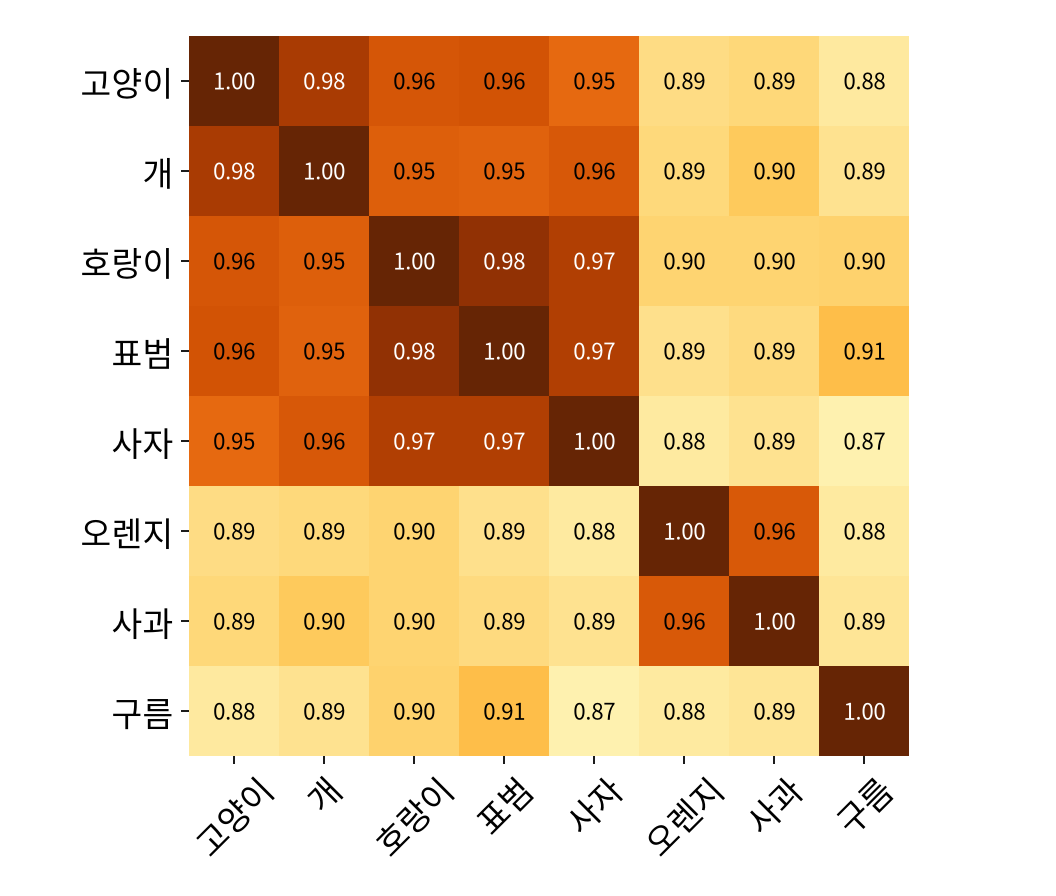
\includegraphics[width=\linewidth]{emb_clip_sim.png}
\column{0.52\linewidth}
{\large CLIP (OpenAI, 2021): 사진-글 \kb{4억} 쌍}\\[0.2em]
{\large 같은 사진 20장씩, 종류별 평균 벡터의 코사인 유사도}\\[0.6em]
{\large 호랑이 $\leftrightarrow$ 표범 \kb{0.98}, \quad 고양이 $\leftrightarrow$ 개 0.98}\\[0.2em]
{\large 오렌지 $\leftrightarrow$ 사과 \kb{0.96}}\\[0.2em]
{\large 과일 $\leftrightarrow$ 동물 0.88 $\sim$ 0.90}\\[0.6em]
{\small 숫자의 크기보다 \textbf{순서}가 중요하다 (CLIP 벡터는 대체로 서로 비슷한 방향)}
\end{columns}
\vfill
\note{두 번째 실험은 많이 배운 임베딩입니다. CLIP은 OpenAI가 2021년에 사진과 그 설명 글 4억 쌍으로 학습한 모델입니다. 같은 CIFAR 사진들을 CLIP에 넣어 종류별 평균 벡터의 코사인 유사도를 쟀습니다. 호랑이와 표범 0.98, 고양이와 개 0.98, 오렌지와 사과 0.96이고, 과일과 동물 사이는 0.88에서 0.90입니다. 이제 오렌지는 사과 곁에, 동물들과는 떨어져 놓입니다. CLIP 벡터는 대체로 비슷한 방향을 향해서 값 자체는 다 높지만, 순서가 중요합니다.}
\end{frame}

% --- 글도 같은 공간에
\begin{frame}{글도 같은 공간에: 0-shot 분류}
\vfill
\centering
{\large 글 ``a photo of a \textbf{tiger}'' 도 같은 공간의 한 점 \quad $\to$ 사진과 가장 가까운 글을 고른다}\vskip0.6em
\renewcommand{\arraystretch}{1.3}
{\large\begin{tabular}{lcccccccc}
 & 고양이 & 개 & 호랑이 & 표범 & 사자 & 오렌지 & 사과 & 구름\\\hline
맞힌 비율 & 95 & 85 & \kq{40} & \kq{30} & 80 & 95 & \kb{100} & \kb{100}
\end{tabular}}\vskip0.6em
{\large 분류 학습 없이 8개 중 평균 \kb{78\%} (찍기 12.5\%)}\\[0.2em]
{\small 32 × 32 작은 사진이라 호랑이 · 표범을 서로 헷갈렸다 \quad 이미지 검색 · 생성 모델 (15주차) 의 바탕}
\vfill
\note{CLIP은 글도 같은 공간에 넣습니다. a photo of a tiger라는 글도 한 점이 되니, 사진과 가장 가까운 글을 고르면 분류가 됩니다. 이 8가지를 따로 학습한 적이 없어서 0-shot 분류라고 합니다. 사과와 구름은 100퍼센트, 고양이와 오렌지는 95퍼센트, 평균 78퍼센트입니다. 찍으면 12.5퍼센트죠. 호랑이와 표범은 40, 30퍼센트로 낮은데, 32 곱하기 32의 작은 사진이라 서로 헷갈린 겁니다. 이렇게 글과 사진을 같은 공간에 두는 임베딩이 이미지 검색과 15주차에 배울 그림 생성 모델의 바탕입니다.}
\end{frame}

% --- 닮음 = 거리
\begin{frame}{닮음을 재는 법: 코사인 유사도}
\vfill
\centering
{\LARGE\[ \cos(\mathbf{a}, \mathbf{b}) = \frac{\mathbf{a} \cdot \mathbf{b}}{\|\mathbf{a}\|\,\|\mathbf{b}\|} \in [-1, 1] \]}\vskip0.2em
{\large 방향만 본다 (길이 무시) \quad 1 = 같은 방향, 0 = 수직, $-1$ = 반대}\\[0.8em]
{\large 예: $\mathbf{a} = (0.7, 0.3)$, $\mathbf{b} = (0.8, 0.1)$ \quad $\to$ \quad $\dfrac{0.56 + 0.03}{0.762 \times 0.806} = \kb{0.96}$}\\[0.6em]
{\large 거리 (유클리드) 도 쓴다: 벡터 길이를 1 로 맞추면 둘은 같은 순서}
\vfill
\note{임베딩끼리 닮음은 주로 코사인 유사도로 잽니다. 두 벡터의 내적을 길이의 곱으로 나눈 값으로, 방향만 보고 길이는 무시합니다. 1이면 같은 방향, 0이면 수직, 마이너스 1이면 반대입니다. 손 계산 표의 3번째 줄 0.7, 0.3과 2번째 줄 0.8, 0.1이면, 내적 0.59를 0.762 곱하기 0.806으로 나눠 0.96입니다. 유클리드 거리도 쓰는데, 벡터 길이를 1로 맞추면 두 방법의 순서가 같아집니다.}
\end{frame}

% --- 쓰임
\begin{frame}{임베딩으로 하는 일}
\vfill
\centering
\renewcommand{\arraystretch}{1.5}
{\large\begin{tabular}{ll}
검색 & 질문 벡터와 가까운 문서 · 사진 찾기 (벡터 데이터베이스)\\
RAG & 챗봇이 답하기 전에 가까운 문서를 찾아 읽는다\\
추천 & 사용자 벡터와 가까운 상품 · 영상\\
전이 학습 & 큰 모델의 임베딩 위에 작은 분류기만 학습\\
이상 탐지 & 어느 무리에서도 먼 점 = 이상한 데이터
\end{tabular}}\vskip0.8em
{\large 공통점: 한 번 숫자로 바꿔 두면 \textbf{가까운 것 찾기}가 된다}
\vfill
\note{임베딩으로 하는 일은 많습니다. 질문의 벡터와 가까운 문서나 사진을 찾는 검색, 챗봇이 답하기 전에 관련 문서를 찾아 읽는 RAG, 사용자 벡터와 가까운 상품을 고르는 추천, 큰 모델의 임베딩 위에 작은 분류기만 학습하는 전이 학습, 어느 무리에서도 먼 점을 찾는 이상 탐지입니다. 공통점은 한 번 숫자로 바꿔 두면 모든 문제가 가까운 것 찾기가 된다는 겁니다.}
\end{frame}

% --- 문제풀이
\begin{frame}{문제풀이}
\vfill
\begin{enumerate}
\item 원-핫 $(0, 1, 0, 0)$ 에 손 계산 표 $W$ 를 곱하면? 단어 3만 개 × 300칸 표의 숫자는 몇 개?\vskip0.8em
\item $\mathbf{a} = (1, 0)$, $\mathbf{b} = (1, 1)$, $\mathbf{c} = (-1, 0)$ 의 코사인 유사도 $\cos(\mathbf{a}, \mathbf{b})$, $\cos(\mathbf{a}, \mathbf{c})$ 는?\vskip0.8em
\item 고양이 · 개만 배운 신경망에서 구름이 99\% 고양이 쪽에 놓였다. 구름이 고양이를 닮았다고 할 수 있나?\vskip0.8em
\item 오렌지와 사과를 구분하는 임베딩이 필요하면 어떤 데이터로 학습해야 할까?
\end{enumerate}
\vfill
\note{1번 답. 표의 2번째 줄, 0.8, 0.1이고, 3만 곱하기 300, 900만 개입니다. 2번 답. a와 b는 1 나누기 루트 2, 약 0.71이고, a와 c는 마이너스 1입니다. 3번 답. 아닙니다. 이 신경망에는 고양이와 개를 가르는 축밖에 없어서, 구름이 어느 쪽에 놓이든 닮음을 뜻하지 않습니다. 4번 답. 과일을 포함한 다양한 사진, 또는 CLIP처럼 사진과 글의 쌍처럼, 구분하고 싶은 차이가 드러나는 데이터로 학습해야 합니다. 임베딩은 배운 과제가 정합니다.}
\end{frame}

% --- 실습
\begin{frame}{실습}
\vfill
\centering\begin{tabular}{rl}
\large 1 & \texttt{nn.Embedding} = 원-핫 × 표, 코사인 유사도 함수\\[0.5em]
\large 2 & 고양이 · 개 CNN 의 임베딩에 처음 보는 사진 넣기 (CIFAR)\\[0.5em]
\large 3 & 문장 임베딩으로 의미 검색 (sentence-transformers, 영어)
\end{tabular}\vskip1em
CIFAR-10 · CIFAR-100 (Krizhevsky 2009) \\[0.4em]\href{https://colab.research.google.com/github/SuminHan/book-ml/blob/main/slides/v2/ml1/week14/embedding/lab/embedding.ipynb}{\textcolor{ksagolddk}{▶ Colab에서 실습 노트북 열기}}
\vfill
\note{실습은 세 부분입니다. 첫째, nn.Embedding이 원-핫 곱하기 표와 같은지 확인하고 코사인 유사도 함수를 만듭니다. 둘째, 고양이와 개만 배운 CNN에 처음 보는 CIFAR-100 사진을 넣어 임베딩이 어디에 놓이는지 봅니다. 셋째, 문장 임베딩 모델로 뜻이 가까운 문장을 찾는 의미 검색을 해 봅니다.}
\end{frame}

% --- 정리
\begin{frame}{정리}
\vfill
\centering\large\begin{tabular}{l}
\textbf{임베딩}: 대상을 숫자 공간의 한 점으로 (표상 = 다시 보여 주기)\\[0.5em]
가장 단순한 꼴: 원-핫 × 표 = 표에서 한 줄 (\texttt{nn.Embedding})\\[0.5em]
고양이 · 개 CNN: 호랑이 83\% 고양이 쪽 \quad 오렌지 · 구름도 억지로 그 축 위에\\[0.5em]
CLIP: 오렌지 $\leftrightarrow$ 사과 0.96, 글과 사진이 한 공간 \quad 닮음 = 코사인 유사도
\end{tabular}
\vfill
\note{정리합니다. 임베딩은 대상을 숫자 공간의 한 점으로 박아 넣은 표상입니다. 가장 단순한 꼴은 원-핫 곱하기 표, 즉 표에서 한 줄을 꺼내는 것입니다. 고양이와 개만 배운 CNN에서 호랑이는 83퍼센트가 고양이 쪽에 놓였지만, 오렌지와 구름도 그 축 위에 억지로 놓였습니다. 임베딩은 배운 만큼만 세상을 보여 줍니다. 4억 쌍으로 배운 CLIP에서는 오렌지가 사과 곁에 놓이고, 글과 사진이 한 공간에 있었습니다. 닮음은 코사인 유사도로 잽니다.}
\end{frame}

% --- 이미지 출처
\begin{frame}{이미지 출처}
\vfill
\begin{itemize}
\item 쇼펜하우어 사진: J. Schäfer (1859), 퍼블릭 도메인 (Wikimedia Commons)
\item 고양이 · 개 · 호랑이 · 표범 · 사자 · 오렌지 · 사과 · 구름 사진: CIFAR-10 · CIFAR-100, A. Krizhevsky (2009) ``Learning Multiple Layers of Features from Tiny Images''
\end{itemize}
\vfill
\end{frame}
\end{document}
